% Generated by documents/paper/figures/make_rq_appendix.py from the rq13_english_only README; do not edit.
\clearpage
\section{English-only models}
\label{app:rq13_english_only}

\paragraph{Question.} The L1 cells are monolingual English. If the trainings are correct they should do clearly better on the (English) benchmarks than the multilingual cells of the same size: higher scores, above chance earlier, and at least as predictable in size, as reliable in their decisions and as high in SNR. Does the ladder show that, and do the L1 numbers land where AllenAI's DataDecide puts the same English tasks?

\paragraph{Setup.} The monolingual-English cells ($L = 1$) against the same-depth baseline cells of every other language setting, which give English half of their tokens; seed 1904, final checkpoints, 90M--1.7B, on the English accuracy tasks above chance at each size.

\paragraph{Key finding.} \textbf{The English-only cells are better at English, by a small margin.} Deep L1 wins more than half of the English accuracy tasks against every other L at every drawn size (25 of 25 (size, L) cells; win share 0.56--0.79 per size, every L pooled), but the mean gap at 1.7B is 1.2 points (33 tasks, every L pooled); shallow L1 wins 28 of 30 cells, 0.6 points at 1.7B. (Figure~\ref{fig:app_rq13_english_only}.)

\begin{figure}[h]
\centering
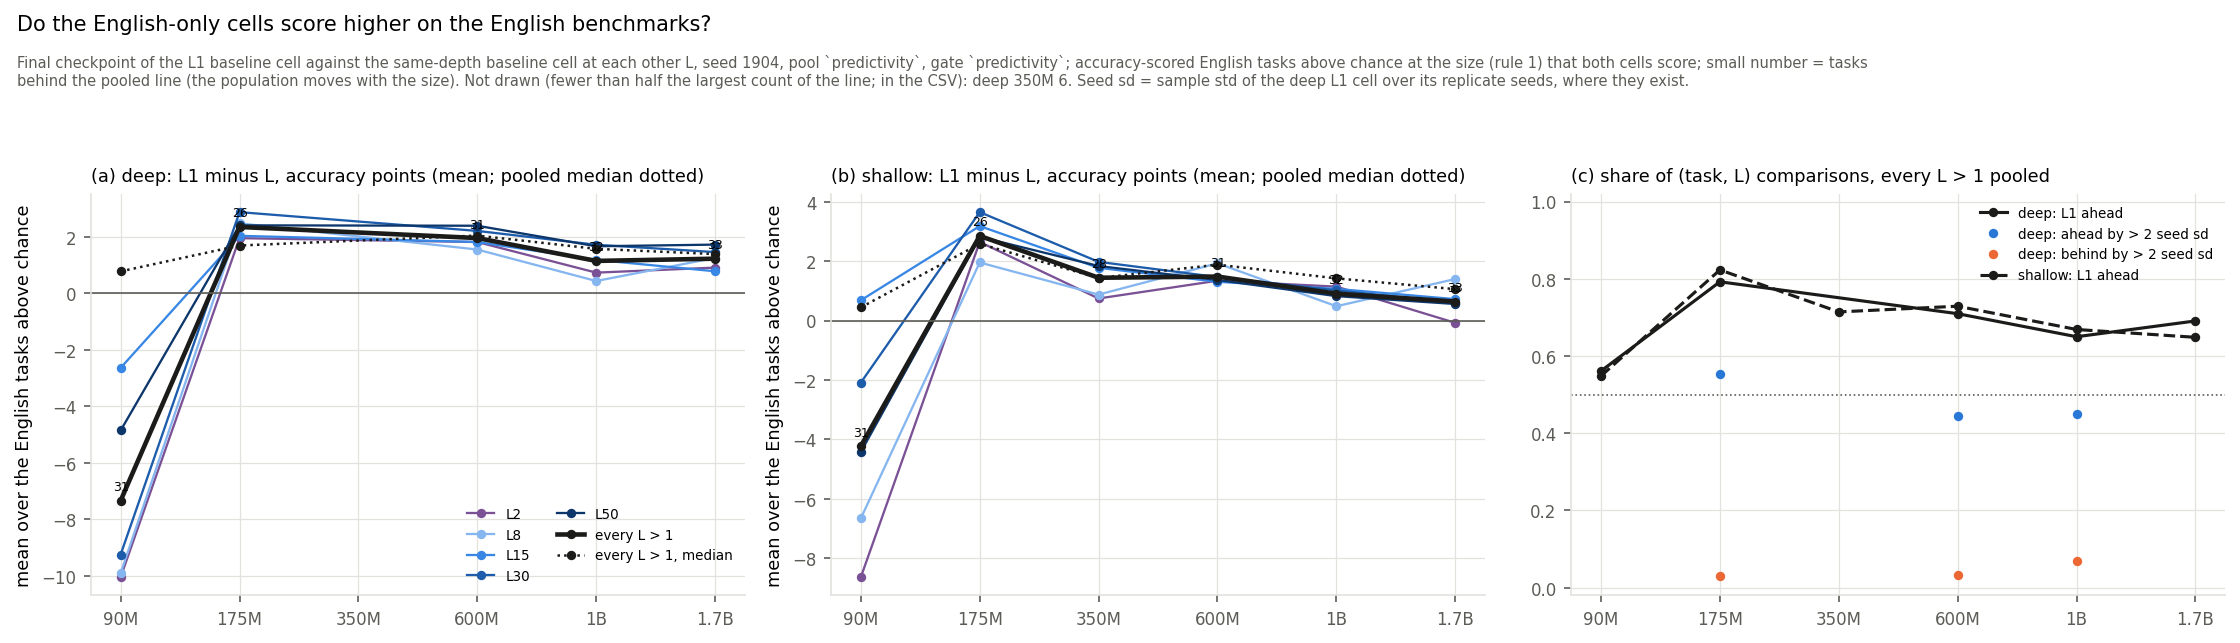
\includegraphics[width=\textwidth]{figures/app_english_only.png}
% source: src/signal-and-noise/analysis/rq13_english_only/pretraining/predictivity/english_only_scores.png
\caption{English benchmark scores of the English-only cells against the multilingual cells of the same size.}
\label{fig:app_rq13_english_only}
\end{figure}
